
Este diagrama ayuda a encontrar si existe una relación entre variables y, de ser así, encontrar una expresión matemática que represente tal relación.

Esta relación puede ser:
\begin{itemize}
    \item Positiva: Una variable aumenta y la otra también
    \item Negativa: Una variable aumenta y la otra disminuye
\end{itemize}

En ambos casos la relación puede ser:

\begin{enumerate}
    \item Fuerte: Una variable aumenta/disminuye mucho y la otra también
    \item Debil: Una variable aumenta/disminuye mucho pero la otra aumenta/disminuye poco
\end{enumerate}

\begin{figure}\centering
    \resizebox{\linewidth}{!}{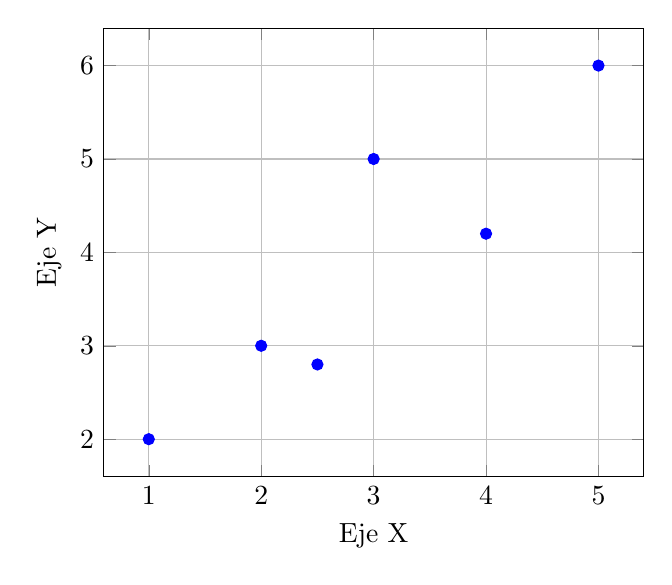
\begin{tikzpicture}
  \begin{axis}[
      xlabel={Eje X},
      ylabel={Eje Y},
      grid=major,
      only marks
    ]
    \addplot[blue, mark=*] coordinates {
      (1, 2) (2, 3) (2.5, 2.8) (3, 5) (4, 4.2) (5, 6)
    };
  \end{axis}
\end{tikzpicture}}
    \rule{\linewidth}{0.5pt}
    \caption{Ejemplo de diagrama de dispersión}
    \label{fig:diagrama_de_dispersion}
\end{figure}

\section{Obtención de modelo matemático}

Para poder obtener el modelo matemático que explique la relación entre variables nos apoyamos de la ecuación de la recta:

\begin{equation}
    y = a_{0} + a_{1}x
\end{equation}

Donde:

\begin{gather}
    a_{1} = \frac{n \sum{x_{i}y_{i}} - (\sum{x_{i}})(\sum{y_{i}}) }{ n \sum{x_{i}^{2}} - (\sum{x_{i}})^{2} }
    \\
    a_{0} = \bar{y} - a_{1}\bar{x}
\end{gather}

Despúes de esto es bueno evaluar cuan bien explica el modelo los datos, lo cual se hace con $r^{2}$ y $r$ ($\sqrt{r^{2}}$)

\begin{equation}
    r = \frac{n \cdot \sum{x_{i}y_{i}} - (\sum{x_{i}}\cdot\sum{y_{i}})}{\sqrt{n\sum{x_{i}^{2}} - (\sum{x_{i}})^{2}} \cdot \sqrt{n\sum{y_{i}^{2}} - (\sum{y_{i}})^{2}}}
\end{equation}

Donde el valor puede ir de -1 a 1, indicando el 0 un ajuste nulo, mientras que -1 y 1 significan un ajuste perfecto.

\section{Linearización}

Si bien mediante lo anterior se nos genera un modelo matemático que sigue una línea recta, cuando los datos están muy poco ajustados a esta linea la capacidad de predicción no es suficiente como para que sea un modelo válido. Para arreglar esto podemos identificar la forma en que se distribuyen los datos y manipularla para que se ajuste mejor a una línea recta, y así aumentar el coeficiente de correlación

Tenemos tres tipos principales de distribuciones:

\begin{itemize}
    \item Exponencial
    \begin{equation}
        y = \alpha \cdot e^{\beta x}
    \end{equation}

    \item Ley de potencias, o potencial
    \begin{equation}
        y = \alpha \cdot x^{\beta}
    \end{equation}

    \item Razón de crecimiento
    \begin{equation}
        y = \alpha \cdot \frac{x}{\beta + x}
    \end{equation}
\end{itemize}

\begin{figure}\centering
    \begin{subfigure}[b]{0.3\linewidth}
        \centering
        \resizebox{\linewidth}{!}{% 2. LEY DE POTENCIAS:  y = α · x^{β}
\begin{tikzpicture}
\begin{axis}[
    width=10cm, height=10cm,
    axis lines=left,
    xlabel={$x$}, ylabel={$y$},
    xtick=\empty, ytick=\empty,
    domain=0:5, samples=50,
    enlargelimits=false,
    legend pos=north west,legend style={draw=none}
]

\pgfmathsetmacro{\myalfa}{3}
\pgfmathsetmacro{\mybeta}{2}

\addplot[DarkRed, thick] {\myalfa*x^\mybeta};
\addlegendentry{\Large $y = \alpha \cdot x^{\beta}$}

\end{axis}
\end{tikzpicture}
}
        \rule{\linewidth}{0.5pt}
        \caption{Modelo potencial}
        \label{fig:modelo_potencial}
    \end{subfigure}
    \hfill
    \begin{subfigure}[b]{0.3\linewidth}\centering
        \resizebox{\linewidth}{!}{\begin{tikzpicture}
\begin{axis}[
    width=10cm, height=10cm,
    axis lines=left,
    xlabel={$x$}, ylabel={$y$},
    xtick=\empty, ytick=\empty,
    xmin=1.5, xmax=5,
    ymin=0, ymax=10,samples=100,
    enlargelimits=false,
    legend pos=north west,legend style={draw=none}
]

\addplot[DarkBlue, thick] {0.5*exp(0.6*x)};
\addlegendentry{\Large $y=\alpha e^{\beta x}$}

\end{axis}
\end{tikzpicture}}
        \rule{\linewidth}{0.5pt}
        \caption{Modelo exponencial}
        \label{fig:modelo_exponencial}
    \end{subfigure}
    \hfill
    \begin{subfigure}[b]{0.3\linewidth}\centering
        \resizebox{\linewidth}{!}{% 3. RAZÓN DE CRECIMIENTO:  y = α · x/(β + x)
\begin{tikzpicture}
\begin{axis}[
    width=10cm, height=10cm,
    axis lines=left,
    xlabel={$x$}, ylabel={$y$},
    xtick=\empty, ytick=\empty,
    domain=0:5, samples=50,
    enlargelimits=false,
    legend pos=south east,legend style={draw=none}
]

\pgfmathsetmacro{\myalfa}{3}
\pgfmathsetmacro{\mybeta}{2}

\addplot[Green, thick] {\myalfa*x/(\mybeta+x)};
\addlegendentry{\Large $y = \alpha \cdot \frac{x}{\beta+x}$}

\end{axis}
\end{tikzpicture}}
        \rule{\linewidth}{0.5pt}
        \caption{Modelo de razon de crecimiento}
        \label{fig:modelo_razon_de_crecimiento}
    \end{subfigure}
    
    \rule{\linewidth}{0.5pt}
    \caption{Ejemplo de cada uno de los modelos}
    \label{fig:modelos}
\end{figure}

Para resolver cada tipo de distribución nos ayudamos de las propiedades de los logaritmos.

\begin{gather}
    \log(a \cdot b) = \log(a) + \log(b)
    \\
    \log \left(\frac{a}{b}\right) = \log(a) - \log(b)
    \\
    \log(a^{b}) = b \cdot \log(a)
    \\
    \log(\sqrt[b]{a}) = \frac{\log(a)}{b}
\end{gather}

\subsection{Exponencial}

\begin{gather}
    \ln(y) = \ln(\alpha \cdot e^{\beta \cdot x})
    \\
    \ln(y) = \ln(\alpha) + \ln(e^{\beta \cdot x})
    \\
    \ln(y) = \ln(\alpha) + \beta \cdot x
    \\
    \hline
    \\
    x = x \quad;\quad y = \ln(y)
    \\
    a_{0} = \ln(\alpha) \quad;\quad a_{1} = \beta
\end{gather}

\subsection{Ley de potencias, o potencial}

\begin{gather}
    \log(y) = \log(\alpha \cdot x^{\beta})
    \\
    \log(y) = \log(\alpha) + \log(x^{\beta})
    \\
    \log(y) = \log(\alpha) + \beta \cdot \log(x)
    \\
    \hline
    \\
    x = \log(x) \quad;\quad y = \log(y)
    \\
    a_{0} = \log(\alpha) \quad;\quad a_{1} = \beta
\end{gather}

\subsection{Razón de crecimiento}

\begin{gather}
    (y)^{-1} = \left(\alpha \cdot \frac{x}{\beta + x}\right)^{-1}
    \\
    \frac{1}{y} = \frac{\beta + x}{\alpha \cdot x}
    \\
    \frac{1}{y} = \frac{\beta \cdot 1}{\alpha \cdot x} + \frac{x}{\alpha \cdot x}
    \\
    \frac{1}{y} = \frac{\beta}{\alpha} \cdot \frac{1}{x} + \frac{1}{\alpha}
    \\
    \hline
    \\
    x = \frac{1}{x} \quad;\quad y = \frac{1}{y}
    \\
    a_{0} = \frac{1}{\alpha} \quad;\quad a_{1} = \frac{\beta}{\alpha}
\end{gather}